\chapter{Les Projets}
\label{Developpement}

\section{MobiSAAS}

\subsection{Cahier des charges, présentation de l'application}

Le projet "MobiSAAS" : MobiAnalyst as a Service, s'inscrit dans la démarche d'entreprise de proposer des solutions en mode \textbf{SAAS}. Le projet consiste d'une manière générale à exposer les fonctionnalités de la solution Desktop du produit "MobiAnalyst"(Fig. \ref{OffreMobiAnalyst}). C'est pour ce projet que j'effectue mon travail de stage.\\

\begin{figure}[!h]
\centering
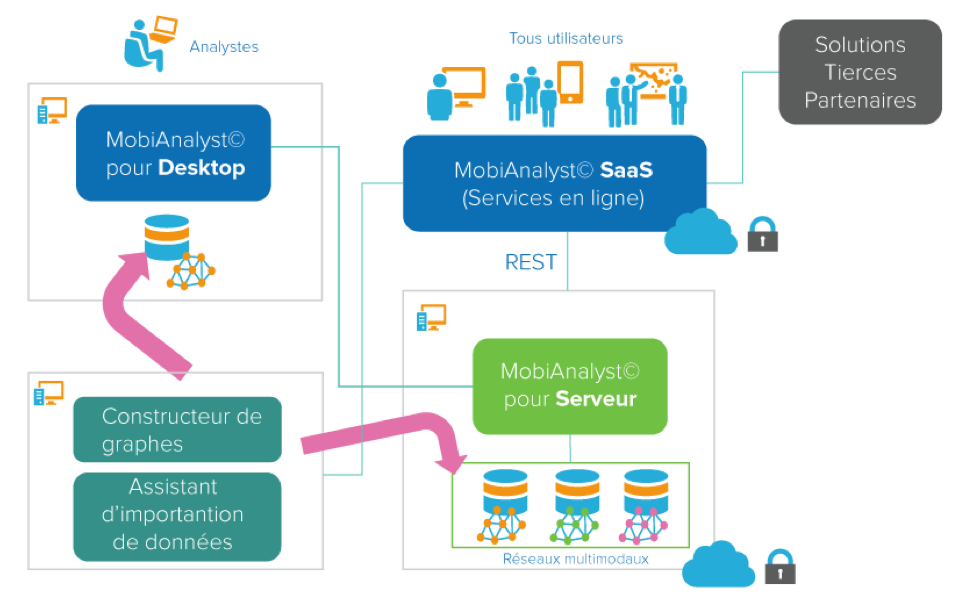
\includegraphics[width=14cm]{images/offre_MobiAnalyst.png}
\caption{\label{OffreMobiAnalyst}Offres du produit MobiAnalyst}
\end{figure} 

\subsubsection{Architecture actuelle}

La figure \ref{fig:architecture} détaille l'ensemble des briques logicielles nécessaires au fonctionnement de la plate-forme MobiSAAS :
\begin{itemize}
\item \textbf{AGS} : ArcGIS Server. Le serveur de Système d'Information Géographique (SIG) permettant de publier et d'administrer des services cartographiques (MapService).
Dans notre cas, les MapServices déployés sont des réseaux routiers et de transport en commun (TC), accompagnés de tables horaires (TimeTable) contenant les horaires des TC.
\item \textbf{SOE}: Server Object Extension. Nous utilisons le mécanisme d'extension "SOE" pour déployer sur un MapService un service spécifique à MobiSAAS. Un SOE est une fonctionnalité qui se déploie sur un MapService et qui expose en Web Service (REST ou SOAP) les solveurs (algorithme de résolution d'itinéraires) de MobiAnalyst.
\item \textbf{MobiAdmin}: Serveur REST d'administration MobiSAAS. Ce serveur (basé sur Java) est le point d'entrée des utilisateurs des services REST de MobiAnalyst.
Il redirige les requêtes métiers vers le bon SOE déployé, il trace ces requêtes et enrichit la base de données client de MobiAnalyst.
L'authentification qui est faite dans les requêtes utilise les comptes d'AGS créés au préalable.
\item \textbf{Postgres} : Système de gestion de base de données. Cette base contient les données clients de MobiAnalyst : profil, traces d'utilisation de MobiSAAS.
\item \textbf{MongoDB} : Système de gestion de base de données. Cette base contient les logs (statistiques mesurées en temps réel) correspondant aux services REST de MobiSAAS.
\end{itemize}\\

\begin{figure}[h]
	\centering
		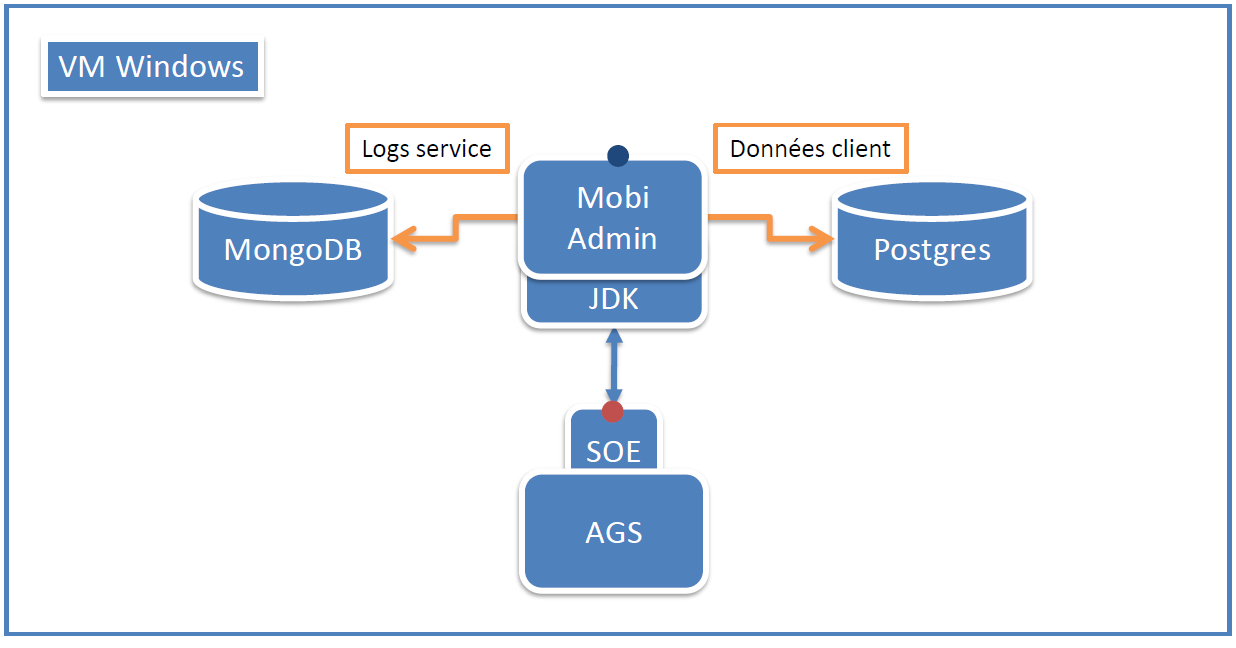
\includegraphics[width=0.8\textwidth]{images/architecture.png}
	\caption{Architecture globale de "MobiAdmin"}
	\label{fig:architecture}
\end{figure}\\

\subsection{Eléments de spécifications fonctionnelles}

Mon stage et les développements demandés concernent le composant d'administration de l'infrastructure : "MobiAdmin". Dans l'objectif de gérer les données du client, je dois proposer un web service pour la gestion des données de transport dans l'espace privatif du client.
La fonctionnalité principale à développer est donc un web service d'upload de données et plus particulièrement l'upload de données de transport public au format GTFS\footnote{\url{https://developers.google.com/transit/gtfs/reference}}.\\ 

L'objectif de ce service d'import de données GTFS est de à plus termes pouvoir manipuler ces données (fichier au format zip), pouvoir récupérer des métadonnées sur les jeux de données exemple : l'extension géographique des données, le nom de l'agence, le nombre de lignes, le mode de transport, et enfin produire un réseau de transport via un service en ligne. Actuellement, ces fonctionnalités sont réalisées en amont du logiciel MobiAnalyst via le logiciel Desktop DataWizard (cf. \ref{DataWizard}).\\

Une archive ou "Upload" de données GTFS peut contenir un seul ou plusieurs jeu de données (ensemble de fichiers .txt). Il faut donc récupérer et renseigner les métadonnées de chaque Upload de fichier :
\begin{itemize}
\item Nom - UUID (identifiant unique)
\item Date d'upload
\item Status d'upload (SUCCESS, FAILED, LOADING, INIT)
\item Nom de l'archive (source)
\item Commentaire libre
\item Chemin vers la données
\item Chemin vers le rapport de validation GTFS
\end{itemsize}\\

Les résultats attendus sont le stockage sur le serveur (système de fichier) des données envoyées par le client, stocker la trace de l'opération dans un SGBD, et enfin la production de réponses HTTP (format JSON) pour chaque requête sur le service.\\

Ce service dédié aux données GTFS est très spécifique. Une attention particulière sera faite afin de développer de manière à abstraire et rendre au maximum générique la plupart des composants afin de proposer d'autres format de données à l'importation sur le serveur REST "MobiAdmin" (utilisation d'interfaces et de classes abstraites).\\

\subsection{Eléments de spécifications techniques}

Pour le composant "MobiAdmin" (serveur REST) qui va héberger les services, le choix technologique majeur est d'utiliser le framework DropWizard (cf. \ref{Dropwizard}). Ce framework orienté microservices nous permet de fournir notamment un serveur embarqué HTTP "Jetty". Et le framework open source Jersey pour la partie webservice REST qui est l'implémentation de référence de la spécification JAX-RS. Ou encore la librairie Jackson "King of JSON" pour la sérialisation/désérialisation du JSON.\\

L'environnement de développement est donc un projet Java EE Maven (cf. \ref{Maven}) composé des éléments de Dropwizard. 
Les \textbf{WS} exposés sont à priori "lourds", sachant qu'un jeu de données peut faire jusqu'à plusieurs centaines de Mo, les opérations de téléchargement, validation, traitement, stockage dans en base,... vont être long à renvoyer une réponse au client après chaque requête. Les WS à développer sont donc asynchrones. De plus, une contrainte supplémentaire est que le service doit supporter plusieurs requêtes simultanées, il faudra donc s'orienter vers un développement en mode "programmation concurrente".\\

\subsubsection{Technologies utilisées}

\textbf{Apache Maven : } \label{Maven}

\begin{wrapfigure}{l}{3cm}
\centering

\includegraphics[width=3cm]{images/apacheMaven.jpg}
\end{wrapfigure}
\noindent C'est un outil pour la gestion et l'automatisation de production des projets logiciels Java en général et Java EE en particulier. L'objectif recherché est comparable au système Make sous Unix : produire un logiciel à partir de ses sources, en optimisant les tâches réalisées à cette fin et en garantissant le bon ordre de fabrication.\\
Il est semblable à l'outil Ant, mais fournit des moyens de configuration plus simples, eux aussi basés sur le format XML. Maven est géré par l'organisation Apache Software Foundation. Précédemment Maven était une branche de l'organisation Jakarta Project.\\
Maven utilise un paradigme connu sous le nom de Project Object Model (POM) afin de décrire un projet logiciel, ses dépendances avec des modules externes et l'ordre à suivre pour sa production. Il est livré avec un grand nombre de tâches pré-définies, comme la compilation de code Java ou encore sa modularisation.\\
Un élément clé et relativement spécifique de Maven est son aptitude à fonctionner en réseau. Une des motivations historiques de cet outil est de fournir un moyen de synchroniser des projets indépendants : publication standardisée d'information, distribution automatique de modules « jar ». Ainsi en version de base, Maven peut dynamiquement télécharger du matériel sur des dépôts logiciels connus. Il propose ainsi la synchronisation transparente de modules nécessaires.\\

Dans le projet MobiSAAS, Maven est très utilisé car c'est un projet multi-modules avec un module parent. Maven me permet donc de télécharger et de gérer les dépendances du projet. Par exemple, voici une extrait du fichier \textbf{POM} du module utilitaire "mobi-admin-util" que j'ai développé (Fig. \ref{fig:MavenPOM}). 
\\
\begin{figure}[h]
	\centering
		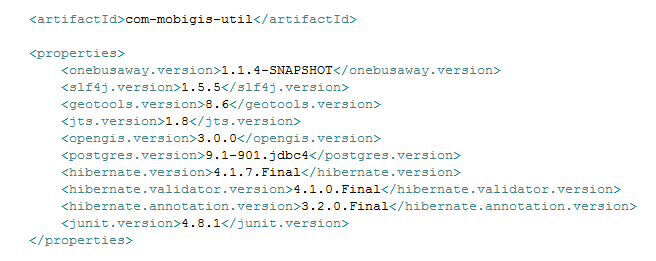
\includegraphics[width=0.8\textwidth]{images/Maven_POM_properties_Mobi-Admin-util.PNG}
	\caption{\label{fig:MavenPOM}Extrait du fichier POM, versions des dépendances utilisées}
\end{figure}\\


\textbf{Dropwizard :}\label{Dropwizard}

\begin{wrapfigure}{l}{3cm}
\centering

\includegraphics[width=3cm]{images/dropwizard.png}
\end{wrapfigure}
\noindent C'est un framework Java léger adapté au développement rapide de microservices REST et ne nécessitant pas de serveur d'application comme environnement d'exécution.
Cela dit, au delà du framework, c'est surtout un assemblage habile de composants spécialisés parmi les meilleurs de l'écosystème Java :
\begin{itemize}
\item \textbf{Jetty}, un serveur HTTP et un moteur de servlet compacts et très performants 
\item \textbf{Jersey}, l'implémentation de référence de la spécification JAX-RS (web services REST) 
\item \textbf{Jackson}, une librairie de sérialisation/dé-sérialisation JSON 
\item \textbf{Hibernate Validator}, l'implémentation de référence de l'API Bean Validation (JSR 303) 
\item \textbf{SLF4J} et \textbf{Logback} pour la gestion des traces 
\item \textbf{Metrics} pour le monitoring 
\item \textbf{jDBI} pour l'interfaçage rapide à une base de données relationnelle. Cette librairie est de bien plus bas niveau que JPA ou Hibernate et présente peu d'abstraction ce qui rend sa prise en main aisée \\
\end{itemize}

Packagée sous la forme d'un jar autonome contenant toutes ses dépendances, l'unité de déploiement n'a pas besoin de serveur d'application pour être exécutée (le conteneur Jetty est embarqué dans le jar). Avec ses 10 Mo tout au plus (dépendances comprises) l'empreinte mémoire d'une application Dropwizard est donc incomparablement plus faible qu'un Web Service SOAP déployé dans un serveur d'application Java EE (jusqu'à plusieurs centaines de Mo).
En conséquences, le temps de démarrage d'une application Dropwizard est de quelques secondes quand il faut parfois plusieurs minutes pour un serveur d'application.\\

On peut considérer ce projet comme une alternative crédible aux serveurs d'applications Java EE perçus comme lourds, compliqués et gourmands en ressources. Le champ des applications couvert par Dropwizard est en réalité plus vaste que celui des microservices (il est tout a fait possible de développer une IHM web) mais l'aisance avec laquelle on développe et déploie un service REST en fait une solution très adaptée à ce type d'usage (à l'instar de Spring Boot de Pivotal ou Spark avec lesquels il est en compétition).\\

La structure d'une application Dropwizard de type API RESTful selon les préconisations d'organisation de projet du framework Dropwizard  (cf. Fig ~\ref{Organisation_Dropwizard}) est : 
\\
\begin{figure}[h]
\centering
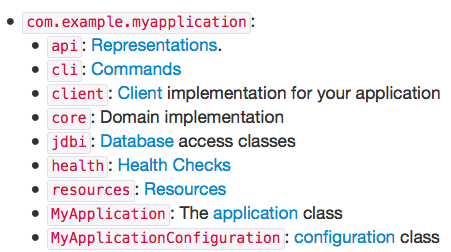
\includegraphics[width=6cm,heigth=6cm]{images/Dropwizard_Project.png}
\caption{\label{Organisation_Dropwizard}Organisation conseillée d'un projet Dropwizard}
\end{figure} 

A partir de cette organisation, nous avons structuré le module "MobiAdmin" comme le montre la figure ci-dessous (cf. Fig ~\ref{Organisation_MobiAdmin}). 
Plusieurs packages spécifiques ou de configuration supplémentaires apparaissent (auth, dao, jsonable, thread,...). 
\\
\begin{figure}[h]
\centering
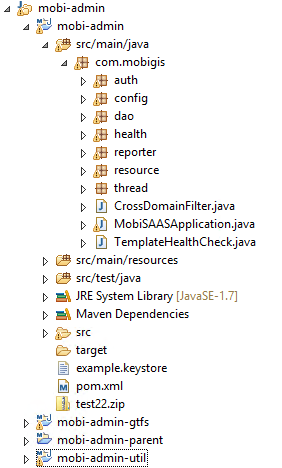
\includegraphics[width=6cm,heigth=6cm]{images/Package_explorer_MobiSAAS.PNG}
\caption{\label{Organisation_MobiAdmin}Organisation du module mobi-admin}
\end{figure} 


A la manière de spring\footnote{\url{http://projects.spring.io/spring-framework/}} un autre framework très utilisé dans les projets Java EE, le code est très simplifié, ainsi le mapping objet-relationnel ou la sérialisation/désérialisation s'en retrouve plus facilement mis en \oe uvre.

\\
\pagebreak

\textbf{Hibernate :}

\begin{wrapfigure}{l}{3cm}
\centering

\includegraphics[width=3cm]{images/hibernate.png}
\end{wrapfigure}
\noindent Dans les langages objet, les données étant le plus souvent stockées dans des bases de données relationnelles ainsi l'utilisation d'un framework de mapping Objet/Relationnel est recommandé pour assurer la rapidité, l'évolutivité et la maintenabilité des développements. Hibernate, issu de la communauté Open Source, répond à ce besoin et connaît depuis quelques années un vif succès. Ce succès s'explique notamment par son architecture parfaitement adaptable à tout type de développements et le support de la majorité des bases de données du marché.\\

Afin de développer les classes pour la gestion des données clients (Uploads) du module «mobi-admin». J'ai mis en place une table «mobiuploads» sur le SGBD PostgreSQL (classes Upload.java, UploadDAO.java).
Grâce au framework Dropwizard, nous avons utilisé Hibernate comme ORM (Object Relationnal Mapping). J'ai pu ainsi manipuler mes objets (opérations CRUD) pour la création, la lecture, la mise à jour et la suppression des objets dans la base. 
Egalement, j'ai développé le chargement de ces données métiers (GTFS) dans le SGBD, j'ai mis en place le modèle de données et développer les classes avec les annotations Hibernate (@Entity, @Table, @JoinColumns,...). Ainsi, si le schéma n'existe pas il se génère automatiquement grâce à Hibernate. 
Toutes les requêtes sont écrites dans les classes java en HQL, langage propre à Hibernate grâce aux annotations @NamedQueries. \\


\textbf{Jackson :}

\begin{wrapfigure}{l}{3cm}
\centering
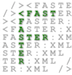
\includegraphics[width=3cm]{images/fxml_logo_Jackson.png}
\end{wrapfigure}
\noindent Jackson est une API JSON, elle est simple, bien documentée, et elle répond aux besoins suivants tels que :
\begin{itemize}
\item Capable de sérialiser et désérialiser des arbres JSON sans adhérence aux beans modèles.
\item Pouvant travailler directement sur des flux.
\item Capable de tenir une charge conséquente, donc stable et performante.
\item Avec le minimum possible de dépendances.
\end{itemize}

Afin que le service puisse renvoyer des réponses convenables et standards nous avons utilisé Jackson via Dropwizard \footnote{\url{http://www.mkyong.com/java/how-to-convert-java-object-to-from-json-jackson/}}. Grâce à la librairie Jackson nous pouvons transformer les "beans" et convertir les propriétés java des objets en éléments Json, ainsi on renvoie par exemple le nom de l'upload, la date d'upload et surtout son status si l'opération c'est bien déroulée ou non (Fig. \ref{fig:Json1}).
\\
\begin{figure}[h]
	\centering
		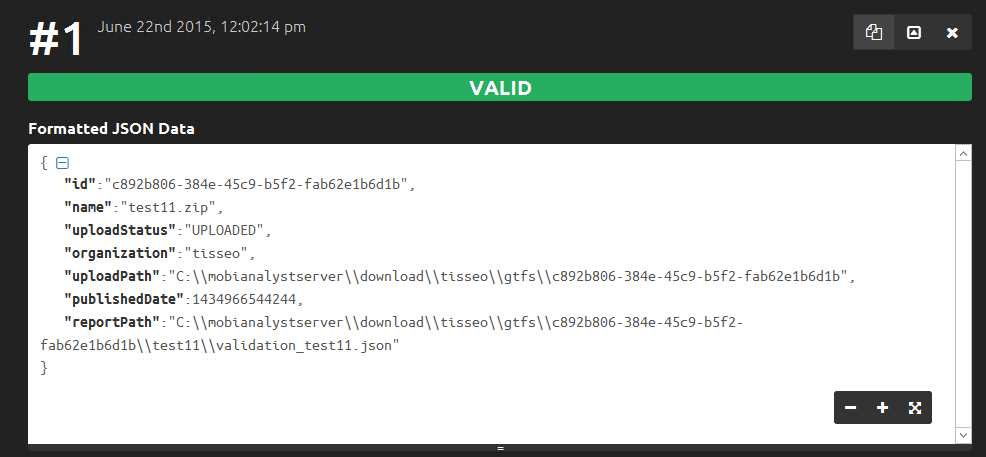
\includegraphics[width=0.8\textwidth]{images/JsonFormatter_serialization.PNG}
	\caption{Réponse Json renvoyée}
	\label{fig:Json1}
\end{figure}\\

De la même manière, chaque donnée GTFS, passe par un traitement métier de validation. Chaque Upload, possède donc une propriété appelée "reportValidationPath" qui indique le chemin vers ce rapport de validation au format json. Ici, Jackson va permettre la production du rapport contenant les métadonnées et les anomalies pour chaque jeu de données GTFS (Fig. \ref{fig:Json2}).
\\
\begin{figure}[h]
	\centering
		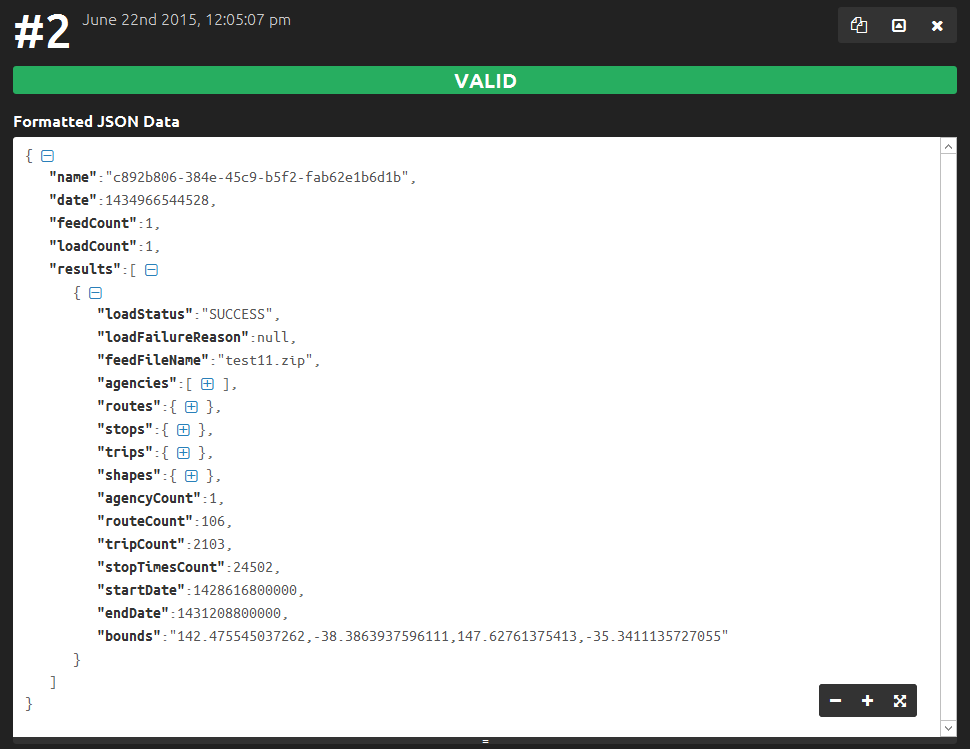
\includegraphics[width=0.8\textwidth]{images/JsonFormatter_serialization_Validation.PNG}
	\caption{Rapport Json de validation des données GTFS}
	\label{fig:Json2}
\end{figure}\\


\textbf{SLF4J et Logback :} 

\begin{wrapfigure}{l}{3cm}
\centering

\includegraphics[width=3cm]{images/slf4j-logo.jpg}

\includegraphics[width=3cm]{images/lblogo.jpg}
\end{wrapfigure}
\noindent SLF4J est une couche d'abstraction pour les API de journalisation Java. Le principe est à peu près similaire à celui de Jakarta Commons Logging. Les avantages de l'utilisation d'une telle couche d'abstraction permettent de s'abstraire de l'implémentation utilisée. Ainsi, il est possible de changer facilement d'implémentation de journalisation sans avoir à toucher la base de code. Au plus, la configuration de l'implémentation de journalisation doit être modifiée. Et enfin, dans le cas de la conception d'une librairie, cela permet de laisser à l'utilisateur de cette librairie le choix du système de journalisation.\\
Logback est un framework de logging. Logback est l'implémentation native de SLF4J, alors que son implémentation pour Log4J (ancêtre de Logback) est « wrappée ». De ce fait, il offre des fonctionnalités supplémentaires à Log4J.\\
Pour la gestion des traces (logs), j'ai donc pour chaque partie du code documenter et produit une trace intelligible à plusieurs niveaux d'informations : INFO, DEBUG, ERROR, etc... Encore une nouvelle fois , via Dropwizard l'utilisation d'un logger est facilité (cf. Extrait du log dans Annexe \ref{Annexe B}).

\textbf{JUnit :} 

\begin{wrapfigure}{l}{3cm}
\centering

\includegraphics[width=3cm]{images/junit-logo.png}
\end{wrapfigure}
\noindent JUnit est un framework de test unitaire por le langage Java, il s'intègre à l'IDE Eclipse. JUnit définit deux types de fichiers de tests. Les TestCase sont des classes contenant un certain nombre de méthodes de tests. Un TestCase sert généralement à tester le bon fonctionnement d'une classe. Une TestSuite permet d'exécuter un certain nombre de TestCase déjà définis. Pour notre cas, nous n'avons utilisé que des TestCase, pour tester de manière unitaire des fonctionnalités. Cet outil a été complémentaire des tests réaliser avec SoapUI.


\subsection{Réalisations}

J'ai tout d'abord commencé par découvrir Maven (cf. \ref{Maven}), les projets, les modules, le désormais célèbre fichier \textbf{POM}, etc...
Ensuite, je me suis documenté sur le code métier existant, et chercher des outils ou librairies de professionnels du domaine (cf. Outils métiers \ref{OBA}).
Enfin, après le "Getting Started" de Dropwizard\footnote{\url{https://dropwizard.github.io/dropwizard/getting-started.html}}, une fois tout cela bien maîtrisé, j'ai pu  commencé la conception et le développement de services web REST.\\

J'ai choisit de stocker les informations concernant ma partie de l'application dans une table PostgreSQL (Fig \ref{TablePostgres})\\
\begin{figure}[!h]
\centering
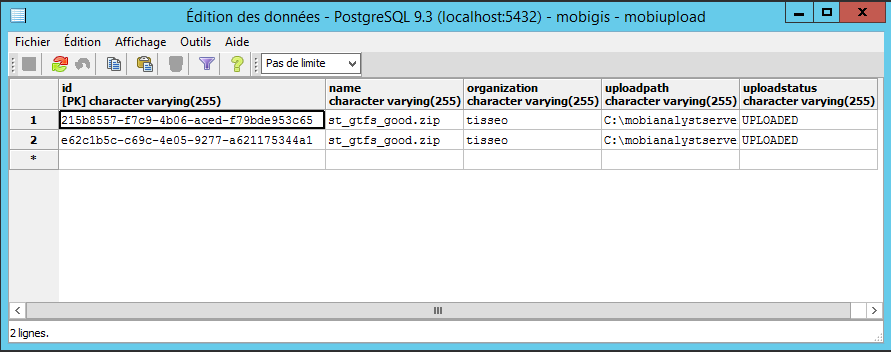
\includegraphics[width=14cm]{images/tablePostgres_mobiupload_small.png}
\caption{\label{TablePostgres}Table des uploads sur le SGBD PostgreSQL}
\end{figure} 

A chaque requête POST du client, je créé une instance d'objet Upload, les informations sont saisies dans la table de suivi, et je stocke les données envoyées sur le serveur. Pour chaque client ou utilisateur, pour chaque type de données, il y a un répertoire personnalisé, chaque upload est "taggé" d'un identifiant unique "UUID".
Le code métier qui a été implémenté est pour le moment le test sur le type de données envoyées, la validation des données et la production d'un rapport d'un validation (JSON), enfin l'extraction (récursive) des données contenues dans l'archive(cf. Annexe \ref{Annexe D}).\\


Exemples de codes DAO :

exemple : UploadDAO

Exemples de codes Persistance /schéma de base de données : 

exemple : compositeKey
exemple : ManyToOne
exemple : com.mobigis.gtfs.model.Agency.java


Exemple de codes métiers :

exemple : GetBoundingBoxGtfs.java (geotools)

exemple : Jackson (ObjectMapper)


Exemple de test unitaires :

exemple : readWriteGTFS.java, completeTestGTFS.java
exemple : GtfsResourceTest.java

\subsection{Perspectives}

L'idéal d'un programme développé dans un langage orienté objet, est la généricité, et la réutilisation d'un maximum de composants. Dans ce travail, l'objectif est clairement de produire un maximum de composant abstrait (classes et interfaces) et de méthodes réutilisables. Les perspectives du projet "MobiSAAS" sont nombreuses : gérer une architecture distribuée, augmenter les fonctionnalités SAAS notamment les principales fonctionnalités du projet "DataWizard".\\

J'ai donc "maquetter l'application" et débuté le développement de ces composants abstraits (ex: Les ressources au sens DropWizard (Fig. \ref{UML1}). Grâce à cela on pourra donc "uploader" plusieurs types de données et réutiliser la méthode manageUpload(). Egalement, sur ce même principe j'ai développé une classe abstaite afin de faire proposer la gestion des threads et tous mes services en hérite, cela limite la duplication de codes dans l'application.\\
\begin{figure}[!h]
\centering
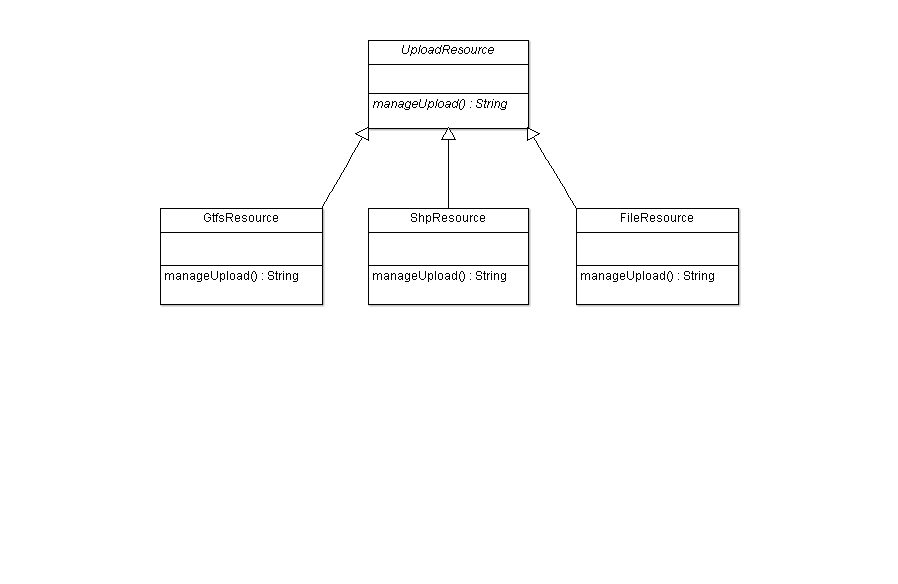
\includegraphics[width=14cm]{images/Diagrammedeclasses_heritage_full.png}
\caption{\label{UML1}Exemple d'abstraction et d'héritage de méthode}
\end{figure} 

\pagebreak

\section{DataWizard}\label{DataWizard}

\subsection{Cahier des charges, présentation de l'application}

Le projet "DataWizard", ensemble de scripts Python et SQL est une application dont le but est d'ingérer des données de transports, et de voirie dans une base de données spatiales (\textbf{PostgreSQL/PostGIS}\ref{Postgis}) afin de produire en sortie un réseau de transport (Network Dataset ou NDS).\\


\subsection{Eléments de spécifications fonctionnelles}

Le DataWizard permet de se lancer par étapes. Il y a 10 étapes successives, dont une étape préliminaire appelée étape 0, et une indépendante : l'étape 10.
\begin{itemize}
\item STEP 0 : Nettoyage et préparation de la base de données
\item STEP 1 : Import des données transport en commun et conversion vers le schéma mobianalyst
\item STEP 2 : Import des données de voirie
\item STEP 3 : Import des données métro et conversion vers le schéma mobianalyst
\item STEP 4 : Génération des données vitesses moyennes et horaires et connexion des réseaux de transport en commun et voirie
\item STEP 5 : Calcul des horaires et des vitesses moyennes
\item STEP 6 : Export des données vers des fichiers Shapefile (.shp)
\item STEP 7 : Import des données dans la Géodatabase de sortie et changement du système de projection si nécessaire
\item STEP 8 : Extraction des différents modes, génération du fichier xml servant à construire le réseau et de MobiNetwork.xml
\item STEP 9 : Construction et compilation du réseau
\item STEP 10 : Production de métadonnées pour le réseau
\end{itemize}

Afin de fournir, un réseau conforme aux attentes du logiciel MobiAnalyst "version 3.0" et des experts en analyse de réseaux de transports, l'équipe me fournit une spécification de métadonnées à extraire des données en entrée du DataWizard (Fig. \ref{DW_Metadata}).\\

\begin{figure}[!h]
\centering
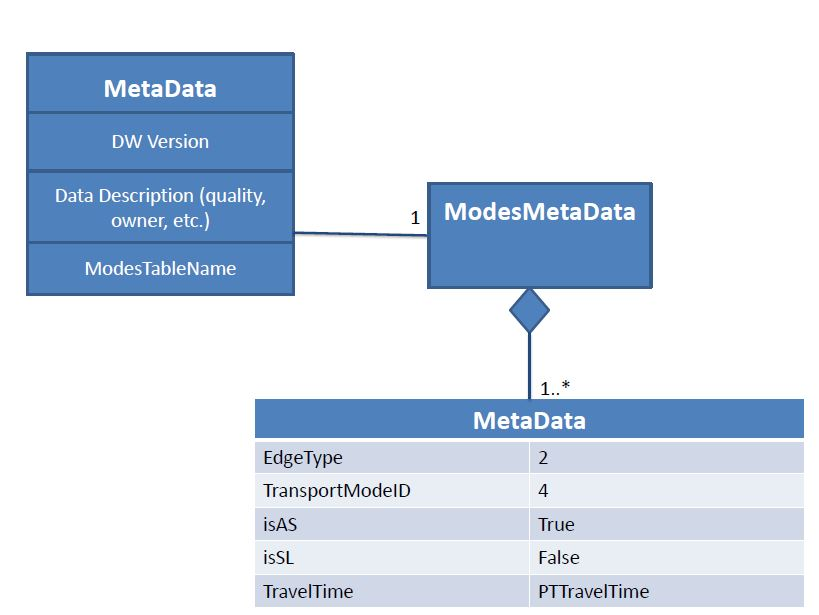
\includegraphics[width=14cm]{images/DW_specMetadata.JPG}
\caption{\label{DW_Metadata}Schéma des tables de métadonnées}
\end{figure} 

\subsection{Eléments de spécifications techniques}

J'intègre tout d'abord le projet en tant qu'utilisateur, j'exploite des données et produits des réseaux de transport en commun (TC) (Bordeaux, Champagne-Ardennes, Montreal, Melbourne,etc...) Ensuite, petit à petit je suis le plan de charge issu du projet Redmine et corrige des bugs, et anomalies.\\

Mon premier travail a été de développer l'étape 10 (STEP 10 : Export Metadata Tables) de l'exécution du DataWizard. Pour cela j'ai du extraire le nombre de mode de transports en commun (variable selon chaque projet), leur code (variable selon chaque projet) et enfin extraire des listes de constantes pour documenter le réseau produit par le DataWizard.\\

Exemple ?\\

Un autre travail réalisé est le développement qui permet la gestion du système de projection des données géographiques pour les calculs du DataWizard. Cette modification impacte quasiment la totalité des requêtes SQL dites spatiales de l'application, et permet des résultats (calculs de distances) plus réalistes (par exemple pour Melbourne, Australie située dans l'hémisphère Sud).\\


\subsection{Réalisations}

Les principales difficultés concernent les données. Ces données sont complexes, les données GTFS ou les données de voirie (données Here (anciennement Navteq) ou OpenStreetMap\footnote{\url{http://openstreetmap.fr/}}). La base de données "DataWizard" possède ainsi de nombreux schémas, et les requêtes SQL sont parfois très complexes mêlant fonctions, et requêtes géographiques.\\

Les résultats obtenus sont la production de nombreux réseaux en version 3.0 (avec les métadonnées) pour nos analystes, et pour les projets nécessitant des réseaux récents (Moveazy, Mobilyse, etc...). Et une version de l'application qui je l'espère est plus stable.\\

Exemple de code pour produire une table de métadonnées (Fig. \ref{CodeMetadata}) :
\\
\begin{figure}[h]
	\centering
		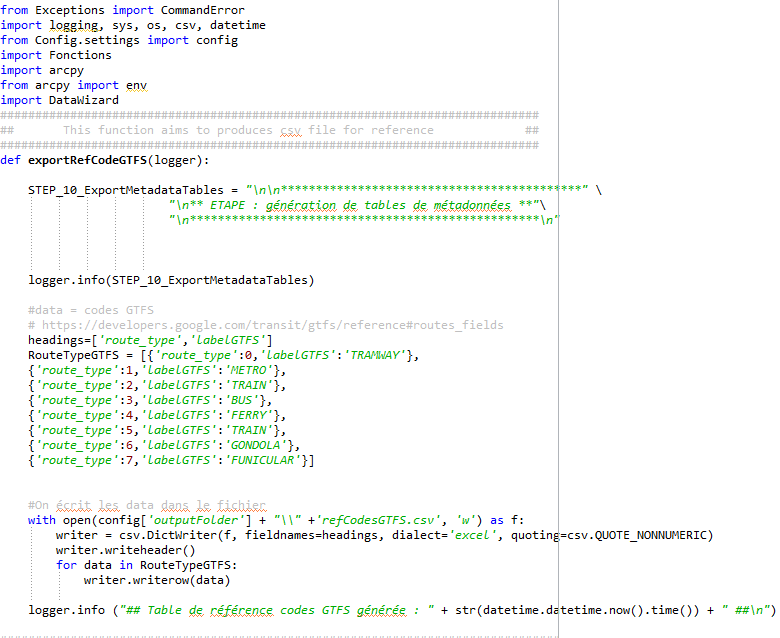
\includegraphics[width=0.8\textwidth]{images/DW_exempleFonctionMetadata.PNG}
	\caption{Exemple de fonction Python pour exporter des métadonnées}
	\label{CodeMetadata}
\end{figure}\\

Dans ce projet, j'ai également développé des fonctions utilitaires : BOMConverter.py, searchAndReplaceFiles.py, etc... Ces méthodes permettent notamment de formater les données avant leur import dans la base de données. Cela peut certainement éviter les mauvaises surprises d'encodage ou de caractères spéciaux fréquemment rencontrés lors de l'exploitation de données GTFS.\\




Exemples langages de bases de données :

exemple requête PostGIS




\subsection{Perspectives}

La liste des évolutions est longue, il y a en effet énormément de perspectives pour le projet... Tout d'abord permettre l'import de plusieurs formats de données, comme l'import de données Shapefile, mais aussi de données de transports en commun "Trident"...
Mais aussi d'une manière générale optimiser les étapes, et développer des routines de simplification de données (afin de ne retenir que les données nécessaires),...\\


\section{Les autres projets}\label{Divers}

\subsection{Crislab}

\subsection{CartoOD}

